\section{BÀI 2. CĂN BẬC BA}
\subsection{Kiến thức trọng tâm}%Minh Quân Fb
\begin{tomtat}
	\subsubsection{Căn bậc ba của một số}
	\begin{itemize}
		\item Cho số thực $a$. Số thực $x$ thỏa mãn $x^3=a$ được gọi là {\it căn bậc ba} của $a$.
		\item Mỗi số thực đều có đúng một căn bậc ba, kí hiệu là $\sqrt[3]{a}$.
		\item Ta luôn có $\left(\sqrt[3]{a}\right)^3=\sqrt[3]{a^3}=a$.
	\end{itemize}
\begin{note}
		Với hai số thực $a$, $b$, ta có
			\begin{itemize}
				\item Nếu $a<b$ thì $\sqrt[3]{a}<\sqrt[3]{b}$;
				\item Nếu $\sqrt[3]{a}<\sqrt[3]{b}$ thì $a<b$;
				\item $a\sqrt[3]{b}=\sqrt[3]{a^3b}$.
			\end{itemize}
\end{note}
	\subsubsection{Căn thức bậc ba}
	Với $A$ là một biểu thức đại số, ta gọi $\sqrt[3]{A}$ là {\bf căn thức bậc ba} của $A$.
	\subsubsection{Tính căn bậc ba của một số bằng máy tính cầm tay}
	Ta có thể sử dụng loại máy tính cầm tay thích hợp để tính căn bậc ba của một số. Chẳng hạn, để tính $\sqrt[3]{343}$ và $\sqrt[3]{12}$ ta làm như sau
	\begin{center}
		\begin{tabular}{|w{c}{2cm}|w{c}{6.5cm}|w{c}{3cm}|}
			\hline
			\textbf{Phép tính} & \textbf{Bấm các phím} & \textbf{Kết quả} \\
			\hline
			$\sqrt[3]{343}$ & \shiftk\key{s}\key{3}\key{4}\key{3}\key{=} & $7$ \\
			\hline
			$\sqrt[3]{12}$ & \shiftk\key{s}\key{1}\key{2}\key{=} & $2{,}289428485$\\
			\hline
		\end{tabular}
	\end{center}
	\begin{luuy}
		Màn hình máy tính cầm tay chỉ hiện thị được một số hữu hạn chữ số nên các kết quả là số thập phân vô hạn (tuần hoàn hoặc không tuần hoàn) đều được làm tròn, chẳng hạn $\sqrt[3]{12}\approx 2{,}289428485$.
	\end{luuy}
\end{tomtat}
%\subsection{Ví dụ}
%Ví dụ 1
\begin{vd}%[Dự án Đề cương Toán 9 CT 2018][Minh Quân Fb]%[9D3N2-1]
	Tìm giá trị của
	\begin{multicols}{2}
		\begin{enumerate}
			\item $\sqrt[3]{1\,000}$;
			\item $\sqrt[3]{-0{,}064}$;
			\item $\sqrt[3]{\dfrac{1}{125}}$;
			\item $\sqrt[3]{-8}$;
			\item $\sqrt[3]{0{,}125}$;
			\item $\sqrt[3]{0}$.
		\end{enumerate}
	\end{multicols}
	\loigiai{
		\begin{multicols}{2}
			\begin{enumerate}
			\item $\sqrt[3]{1\,000}=\sqrt[3]{10^3}=10$.
			\item $\sqrt[3]{-0{,}064}=\sqrt[3]{(-0{,}4)^3}=-0{,}4$.
			\item $\sqrt[3]{\dfrac{1}{125}}=\sqrt[3]{\left(\dfrac{1}{5}\right)^3}=\dfrac{1}{5}$.
			\item $\sqrt[3]{-8}=\sqrt[3]{(-2)^3}=-2$.
			\item $\sqrt[3]{0{,}125}=\sqrt[3]{(0{,}5)^3}=0{,}5$.
			\item $\sqrt[3]{0}=0$.
		\end{enumerate}
\end{multicols}
	}
\end{vd}
%Ví dụ 2
\begin{vd}%[Dự án Đề cương Toán 9 CT 2018][Minh Quân Fb]%[9D3N2-1]
	So sánh 
	\begin{multicols}{2}
		\begin{enumerate}
			\item $\sqrt[3]{5}$ và $\sqrt[3]{4}$;
			\item $\sqrt[3]{5}$ và $2$;
			\item $4\sqrt[3]{5}$ và $5\sqrt[3]{4}$;
			\item $\sqrt[3]{5}+\sqrt[3]{7}$ và $\sqrt[3]{12}$.
	\end{enumerate}
	\end{multicols}  
	\loigiai{
		\begin{enumerate}
			\item Ta có $4<5$, suy ra $\sqrt[3]{4}<\sqrt[3]{5}$.
			\item Ta có $8>5$, suy ra $\sqrt[3]{8}>\sqrt[3]{5}$, do đó $2>\sqrt[3]{5}$.
			\item Ta có $5\sqrt[3]{4}=\sqrt[3]{5^3 \cdot 4} = \sqrt[3]{500}$ và $4\sqrt[3]{5}=\sqrt[3]{4^3\cdot 5}=\sqrt[3]{320}$.\\
			Vì $\sqrt[3]{320}<\sqrt[3]{500}$ nên $4\sqrt[3]{5}<5\sqrt[3]{4}$.
			\item Ta có $\left(\sqrt[3]{5}+\sqrt[3]{7}\right)^3=5+3\sqrt[3]{5^2\cdot 7}+3\sqrt[3]{5\cdot 7^2}+7=12+3\sqrt[3]{175}+3\sqrt[3]{245}$ và
				$\left(\sqrt[3]{12}\right)^3=12$.\\
				Vì $12+3\sqrt[3]{175}+3\sqrt[3]{245}>12$ nên  $\sqrt[3]{5}+\sqrt[3]{7}>\sqrt[3]{12}$.
		\end{enumerate}	

	}
\end{vd}
%Ví dụ 3
\begin{vd}%[Dự án Đề cương Toán 9 CT 2018][Minh Quân Fb]%[9D3H2-3]
	Rút gọn các biểu thức
	\begin{multicols}{2}\begin{enumerate}
			\item $5\sqrt[3]{128}+3\sqrt[3]{16}$;
			\item $\sqrt[3]{a^9}$;
			\item $\sqrt[3]{-8x^6}$;
			\item  $-x+5+\sqrt[3]{x^3+3x^2+3x+1}$;
			\item $\sqrt[3]{x^3-3x^2+3x-1}$.
	\end{enumerate}\end{multicols}
	\loigiai{
		\begin{enumerate}
			\item Ta có
			\begin{eqnarray*}
				5\sqrt[3]{128}+3\sqrt[3]{16}&=&  5 \sqrt[3]{64\cdot2}+3\sqrt[3]{8\cdot2}	\\
				&=& 5\sqrt[3]{4^3\cdot 2}+3 \sqrt[3]{2^3 \cdot 2}  \\
				&=& 5\sqrt[3]{4^3}\cdot \sqrt[3]{2}+3\sqrt[3]{2^3}\cdot\sqrt[3]{2}  \\
				&=& 5\cdot 4 \sqrt[3]{2}+3\cdot 2\sqrt[3]{2}  \\
				&=&  20\sqrt[3]{2}+6\sqrt[3]{2} \\
				&=&  26\sqrt[3]{2}.
			\end{eqnarray*}
			Vậy $5\sqrt[3]{128}+3\sqrt[3]{16}=26 \sqrt[3]{2}$.
			\item Ta có $\sqrt[3]{a^9}=\sqrt[3]{(a^3)^3}=a^3$.
			\item Ta có $\sqrt[3]{-8x^6}=\sqrt[3]{-8}\cdot\sqrt[3]{x^6}=\sqrt[3]{(-2)^3}\cdot\sqrt[3]{(x^2)^3}=(-2)\cdot x^2=-2x^2$.
			\item Ta có $x^3+3x^2+3x+1=(x+1)^3$.\\
			Do đó $-x+5+\sqrt[3]{x^3+3x^2+3x+1}=-x+5+\sqrt[3]{(x+1)^3}=-x+5+x+1=6$.
			\item Ta có $x^3-3x^2+3x-1=(x-1)^3$.\\
			Do đó $\sqrt[3]{x^3-3x^2+3x-1}=\sqrt[3]{(x-1)^3}=x-1$.
		\end{enumerate}
	}
\end{vd}
%%===Ví dụ 4
\begin{vd}%[Dự án Đề cương Toán 9 CT 2018][Minh Quân Fb]%[9D3H2-3]
	Tính giá trị của căn thức $\sqrt[3]{2x+5}$ tại
	\begin{multicols}{2}		
		\begin{enumerate}
			\item $x=60$;
			\item $x=-6{,}5$.
	\end{enumerate}	\end{multicols}
	\loigiai{
		\begin{enumerate}
			\item Với $x=60$ ta có $\sqrt[3]{2\cdot 60+5}=\sqrt[3]{125}=\sqrt[3]{5^3}=5$.
			\item Với $x=-6{,}5$ ta có $\sqrt[3]{2\cdot (-6{,}5)+5}=\sqrt[3]{-8}=\sqrt[3]{(-2)^3}=-2$.
		\end{enumerate}
	}
\end{vd}
%Ví dụ 5
\begin{vd}%[Dự án Đề cương Toán 9 CT 2018][Minh Quân Fb]%[9D3H2-3]
	Cho biểu thức $Q=\sqrt[3]{3x^2}$. Tính giá trị của $Q$ khi $x=2$ và khi $x=-3$ (kết quả làm tròn đến chữ số thập phân thứ hai).
	\loigiai{
		\begin{itemize}
			\item Với $x=2$, ta có $Q=\sqrt[3]{3\cdot 2^2}=\sqrt[3]{12}\approx 2{,}29$.
			\item Với $x=-3$, ta có $Q=\sqrt[3]{3\cdot (-3)^2}=\sqrt[3]{27}=3$.
		\end{itemize}
	}
\end{vd}
%Ví dụ 6
\begin{vd}%[Dự án Đề cương Toán 9 CT 2018][Minh Quân Fb]%[9D3H2-2]
	Sử dụng máy tính cầm tay, tìm căn bậc ba của các số sau (kết quả làm tròn đến chữ số thập phân thứ ba).
		\begin{multicols}{4}		
			\begin{enumerate}
		\item $25$;
		\item $-100$;
		\item $8{,}5$;
		\item $\dfrac{1}{5}$.
\end{enumerate}	\end{multicols}
	\loigiai{
		\begin{enumerate}
			\item Để tính $\sqrt[3]{25}$, ấn liên tiếp các nút 
			\key{q}\key{s}\key{2}\key{5}\key{=} ta được kết quả $2{,}9240177$.\\
			Từ đó, $\sqrt[3]{25}\approx 2{,}924$ (kết quả làm tròn đến chữ số thập phân thứ ba).
			\item Để tính $\sqrt[3]{-100}$, ấn liên tiếp các nút 
			\key{q}\key{s}\key{z}\key{1}\key{0}\key{0}\key{=} ta được kết quả $-4{,}641589$.\\
			Từ đó, $\sqrt[3]{-100}\approx -4{,}642$ (kết quả làm tròn đến chữ số thập phân thứ ba).
			\item Để tính $\sqrt[3]{8{,}5}$, ấn liên tiếp các nút 
			\key{q}\key{s}\key{8}\key{.}\key{5}\key{=} ta được kết quả $2{,}0408276$.\\
			Từ đó, $\sqrt[3]{8{,}5}\approx 2{,}041$ (kết quả làm tròn đến chữ số thập phân thứ ba).
			\item Để tính $\sqrt[3]{\dfrac{1}{5}}$, ấn liên tiếp các nút 
			\key{q}\key{s}\key{1}\key{a}\key{5}\key{=} ta được kết quả $0{,}58480355$.\\
			Từ đó, $\sqrt[3]{\dfrac{1}{5}}\approx 0{,}485$ (kết quả làm tròn đến chữ số thập phân thứ ba).
		\end{enumerate}
	}
\end{vd}
%Ví dụ 7
\begin{vd}%[Dự án Đề cương Toán 9 CT 2018][Minh Quân Fb]%[9D3H2-3]
	Tìm $x$ biết
	\begin{multicols}{4}		
	\begin{enumerate}
		\item $x^3=-27$;
		\item $x^3=\dfrac{64}{125}$;
		\item $\sqrt[3]{x}=8$;
		\item $\sqrt[3]{x}=-0{,}9$.
\end{enumerate}	\end{multicols}
	\loigiai{
	\begin{enumerate}
			\item Vì $x^3=-27$ nên $x^3=(-3)^3$, suy ra $x=-3$.
			\item Vì $x^3=\dfrac{64}{125}$ nên $x^3=\left(\dfrac{4}{5}\right)^3$, suy ra $x=\dfrac{4}{5}$.
			\item Vì $\sqrt[3]{x}=8$ nên $\left(\sqrt[3]{x}\right)^3=8^3$, suy ra $x=512$.
			\item Vì $\sqrt[3]{x}=-0{,}9$ nên $\left(\sqrt[3]{x}\right)^3=(-0{,}9)^3$, suy ra $x=-0{,}729$.
	\end{enumerate}
	}
\end{vd}
%Ví dụ 8
\begin{vd}%[Dự án Đề cương Toán 9 CT 2018][Minh Quân Fb]%[9D3V3-4]
	\immini{
		Bán kính $r$ (m) của quỹ đạo của một vệ tinh (giả sử quỹ đạo của vệ tinh là đường tròn) được ước tính bởi công thức $r=\sqrt[3]{\dfrac{GMt^2}{4\pi^2}}$, trong đó $G$ (Nm$^2$/kg$^2$) là hằng số hấp dẫn vũ trụ, $M$ (kg) là khối lượng của Trái Đất và $t$ (s) là thời gian để vệ tinh hoàn thành một quỹ đạo. {\it (nguồn: https://courses.lumenlearning.com/suny-osuniversityphysics/chapter/13-4-satellite-orbitsand-energy/)}.\\
		Hãy ước tính bán kính của quỹ đạo của vệ tinh có thời gian hoàn thành một quỹ đạo là $2{,}6\cdot 10^6$ giây, biết rằng $G=\dfrac{6{,}67}{10^{11}}$ (Nm$^2$/kg$^2$) và $M=5{,}98\cdot10^{24}$ (kg) (làm tròn kết quả đến hàng nghìn).
	}{
		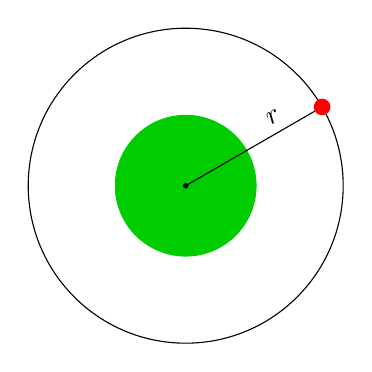
\begin{tikzpicture}[declare function={r=3;}]
			\path (0:0) coordinate (O)
			(30:0.9r) coordinate (A)
			(30:2r) coordinate (B);
			\fill[green!80!black] (O) circle (0.9r);
			\draw (O)--(B)node[pos=.7, sloped, above]{$r$};
			\draw (O) circle (2r);
			\fill (O) circle (1pt);
			\fill[red] (B) circle (3pt);
		\end{tikzpicture}
	}
	\loigiai{
		Bán kính của quỹ đạo của vệ tinh là
		\begin{eqnarray*}
			r=\sqrt[3]{\dfrac{\dfrac{6{,}67}{10^{11}}\cdot5{,}98\cdot10^{24}\cdot \left(2{,}6\cdot 10^6\right)^2}{4 \pi^2}}\approx408\,763\,000 \text{ (m)}.
		\end{eqnarray*}
	}
\end{vd}
\subsection{Bài tập}
%Bài 1
\begin{bt}%[Dự án Đề cương Toán 9 CT 2018][Minh Quân Fb]%[9D3N2-1]
	Tính giá trị của các căn thức bậc ba
	\begin{multicols}{2}	\begin{enumerate}
			\item $\sqrt[3]{64}$;
			\item $\sqrt[3]{-512}$;
			\item $\sqrt[3]{0{,}064}$;
			\item $\sqrt[3]{-0{,}216}$.
	\end{enumerate} \end{multicols}
	\loigiai{
		\begin{enumerate}
			\item $\sqrt[3]{64}=\sqrt[3]{(4)^3}=4$.
			\item $\sqrt[3]{-512}=\sqrt[3]{(-8)^3}=-8$.
			\item $\sqrt[3]{0{,}064}=\sqrt[3]{\dfrac{64}{1\,000}}=\dfrac{\sqrt[3]{64}}{\sqrt[3]{1\,000}}=\dfrac{\sqrt[3]{(4)^3}}{\sqrt[3]{(10)^3}}=\dfrac{4}{10}=\dfrac{2}{5}$.
			\item $\sqrt[3]{-0{,}216}=\sqrt[3]{(-0{,}6)^3}=-0{,}6$.
		\end{enumerate}
	}
\end{bt}
%Bài 2
\begin{bt}%[Dự án Đề cương Toán 9 CT 2018][Minh Quân Fb]%[9D3H2-1]
	So sánh
	\begin{multicols}{2}	\begin{enumerate}
			\item $\sqrt[3]{9}$ và $2$;
			\item $\sqrt[3]{\dfrac{1}{8}}$ và $\dfrac{3}{4}$;
			\item $2\sqrt[3]{3}$ và $3\sqrt[3]{2}$;
			\item $-6\sqrt[3]{7}$ và $7\sqrt[3]{\left(-6\right)}$;
			\item $\sqrt[3]{4}+\sqrt[3]{7}$ và $\sqrt[3]{11}$;
			\item $\sqrt[3]{10}-2$ và $ \sqrt[3]{2}$;
			\item $\sqrt{2}+1$ và $\sqrt[3]{7+5\sqrt{2}}$;
			\item $\sqrt{3}-2$ và $\sqrt[3]{15\sqrt{3}-25}$.
		\end{enumerate}	\end{multicols}
	\loigiai{
		\begin{enumerate}
			\item Ta có $2=\sqrt[3]{8}$. Vì $\sqrt[3]{8}<\sqrt[3]{9}$ nên $\sqrt[3]{9}>2$.
			\item Ta có $\sqrt[3]{\dfrac{1}{8}}=\sqrt[3]{\left(\dfrac{1}{2}\right)^3}=\dfrac{1}{2}<\dfrac{3}{4}$. Do đó $\sqrt[3]{\dfrac{1}{8}}<\dfrac{3}{4}$.
			\item Ta có $2\sqrt[3]{3}=\sqrt[3]{2^3\cdot 3}=\sqrt[3]{24}$ và $3\sqrt[3]{2}=\sqrt[3]{3^3\cdot 2}=\sqrt[3]{54}$.\\
			Vì $\sqrt[3]{24}<\sqrt[3]{54}$ nên $2\sqrt[3]{3}<3\sqrt[3]{2}$.
			\item Ta có $-6\sqrt[3]{7}=\sqrt[3]{(-6)^3\cdot 7}=\sqrt[3]{-1\,512}$ và $7\sqrt[3]{(-6)}=\sqrt[3]{7^3\cdot (-6)} = \sqrt[3]{-2\,058}$.\\
			Từ đó suy ra $-6\sqrt[3]{7}>7\sqrt[3]{(-6)}$.
			\item Ta có $\left(\sqrt[3]{4}+\sqrt[3]{7}\right)^3= 4+3\sqrt[3]{112}+3\sqrt[3]{196}+7=11+3\sqrt[3]{112}+3\sqrt[3]{196}
			>11=\left(\sqrt[3]{11}\right)^3$.\\
			Từ đó suy ra $\sqrt[3]{4}+\sqrt[3]{7}>\sqrt[3]{11}$.
			\item Ta có $\left(\sqrt[3]{10}\right)^3 = 10$ và $\left(\sqrt[3]{2}+2 \right)^3=2+6\sqrt[3]{4}+12\sqrt[3]{2}+8=10+6\sqrt[3]{4}+12\sqrt[3]{2}$.\\
			Từ đó suy ra
			\begin{eqnarray*}
				\left(\sqrt[3]{10}\right)^3 &<& \left(\sqrt[3]{2}+2 \right)^3 \\
				\sqrt[3]{10} &<& \sqrt[3]{2}+2 \\
				\sqrt[3]{10}-2	&<& \sqrt[3]{2}.
			\end{eqnarray*}
			\item Ta có $\left(\sqrt{2}+1\right)^3=2\sqrt{2}+6+3\sqrt{2}+1=7+5\sqrt{2}$.\\
			Từ đó suy ra $\sqrt{2}+1=\sqrt[3]{7+5\sqrt{2}}$.
			\item Ta có $\left(\sqrt{3}-2\right)^3=3\sqrt{3}-18+12\sqrt{3}-8=15\sqrt{3}-26<15\sqrt{3}-25$.\\
			Từ đó suy ra $\sqrt{3}-2<\sqrt[3]{15\sqrt{3}-25}$.
		\end{enumerate}
	}
\end{bt}

%Bài 4
\begin{bt}%[Dự án Đề cương Toán 9 CT 2018][Minh Quân Fb]%[9D3H2-3]
	Rút gọn các biểu thức
	\begin{multicols}{3}\begin{enumerate}
			\item $\sqrt[3]{\left(1-\sqrt{2}\right)^3}$;
			\item $\sqrt[3]{\left(2\sqrt{2}+1\right)^3}$;
			\item $\left(\sqrt[3]{\sqrt{2}+1}\right)^3$;
			\item $\sqrt[3]{m^6}$;
			\item $\sqrt[3]{-27n^3}$;
			\item $\sqrt[3]{64y^3}-7y$.
	\end{enumerate}\end{multicols}
	\loigiai{
		\begin{multicols}{2}\begin{enumerate}
			\item $\sqrt[3]{\left(1-\sqrt{2}\right)^3}=1-\sqrt{2}$;
			\item $\sqrt[3]{\left(2\sqrt{2}+1\right)^3}=2\sqrt{2}+1$;
			\item $\left(\sqrt[3]{\sqrt{2}+1}\right)^3=\sqrt{2}+1$;
			\item $\sqrt[3]{m^6}=\sqrt[3]{\left(m^2\right)^3}=m^2$;
			\item $\sqrt[3]{-27n^3}=\sqrt[3]{(-3n)^3}=-3n$;
			\item $\sqrt[3]{64y^3}-7y=\sqrt[3]{(4y)^3}-7y=4y-7y=-3y$.
	\end{enumerate}\end{multicols}
	}
\end{bt}

%Bài 5
\begin{bt}%[Dự án Đề cương Toán 9 CT 2018][Minh Quân Fb]%[9D3H2-3]
	Tính giá trị của biểu thức $P=\sqrt[3]{64n}$ khi $n=1$; $n=-1$; $n=\dfrac{1}{125}$.
	\loigiai{
		\begin{itemize}
			\item Với $n=1$, ta có $P=\sqrt[3]{64\cdot 1}=\sqrt[3]{64}=\sqrt[3]{4^3}=4$.
			\item Với $n=-1$, ta có $P=\sqrt[3]{64\cdot (-1)}=\sqrt[3]{-64}=\sqrt[3]{(-4)^3}=-4$.
			\item Với $n=\dfrac{1}{125}$, ta có $P=\sqrt[3]{64\cdot \dfrac{1}{125}}=\sqrt[3]{\dfrac{64}{125}}=\sqrt[3]{\left(\dfrac{4}{5}\right)^3}=\dfrac{4}{5}$.
		\end{itemize}
	}
\end{bt}
%Bài 5
\begin{bt}%[Dự án Đề cương Toán 9 CT 2018][Minh Quân Fb]%[9D3H2-3]
	Tìm $x$, biết rằng
	\begin{multicols}{2}\begin{enumerate}
			\item $\sqrt[3]{x-2}=3$;
			\item $6x+\sqrt[3]{-8x^3}=2x+1$;
			\item $x^3=-0,027$;
			\item $\sqrt[3]{x}=-\dfrac{2}{3}$;
			\item $\sqrt[3]{x+7}-3=1$;
			\item $\sqrt[3]{1\,000x}-\sqrt[3]{64x}-\sqrt[3]{27x}=15$;
			\item $\sqrt[3]{x}+\sqrt[3]{x+1}+\sqrt[3]{x+2}=0$.
	\end{enumerate}\end{multicols}
	\loigiai{
		\begin{enumerate}
			\item Ta có
			\begin{eqnarray*}
				\sqrt[3]{x-2}&=&3	\\
				{x-2}&=&3^3	\\
				{x-2}&=&27 \\
				x&=&27+2\\
				x&=&29.
			\end{eqnarray*}
			Vậy $x=29$.
			\item Ta có
			\begin{eqnarray*}
				6x+\sqrt[3]{-8x^3}&=&2x+1	\\
				\sqrt[3]{-8x^3}&=&2x+1-6x  	\\
				\sqrt[3]{(-2x)^3}&=& -4x+1  \\
				-2x&=& -4x+1   \\
				2x&=&1   \\
				x&=&\dfrac{1}{2}. 
			\end{eqnarray*}
			Vậy $x=\dfrac{1}{2}$.
			\item Ta có
			\begin{eqnarray*}
				x^3&=&-0{,}027\\
				x&=&\sqrt[3]{-0{,}027}\\
				x&=&-0{,}3.
			\end{eqnarray*}
			Vậy $x=-0{,}3$.
			\item Ta có
			\begin{eqnarray*}
				\sqrt[3]{x}&=&-\dfrac{2}{3}\\
				x&=&\left(-\dfrac{2}{3}\right)^3\\
				x&=&-\dfrac{8}{27}.
			\end{eqnarray*}
			Vậy $x=-\dfrac{8}{27}$.
			\item Ta có
			\begin{eqnarray*}
				\sqrt[3]{x+7}-3	&=& 1 \\
				\sqrt[3]{x+7}	&=& 4 \\
				x+7	&=& 64 \\
				x	&=& 57.
			\end{eqnarray*}
			Vậy $x=57$.
			\item Ta có
			\begin{eqnarray*}
				\sqrt[3]{1\,000x}-\sqrt[3]{64x}-\sqrt[3]{27x}	&=& 15 \\
				10\sqrt[3]{x}-4\sqrt[3]{x}-3\sqrt[3]{x}	&=& 15 \\
				\sqrt[3]{x}	&=& 5 \\
				x	&=& 125.
			\end{eqnarray*}
			Vậy $x=125$.
			\item Ta có
			\begin{eqnarray*}
				\sqrt[3]{x}+\sqrt[3]{x+1}+\sqrt[3]{x+2}	&=&0 \\
				\sqrt[3]{x}+\sqrt[3]{x+1}&=&-\sqrt[3]{x+2}. \\
				x+x+1+3\sqrt[3]{x(x+1)}\left(\sqrt[3]{x}+\sqrt[3]{x+1}\right)	&=& -x-2\\
				3x+3+3\sqrt[3]{x(x+1)}\left(\sqrt[3]{x}+\sqrt[3]{x+1}\right)	&=& 0\\
				3x+3+3\sqrt[3]{x(x+1)}\left(-\sqrt[3]{x+2}\right)	&=& 0\\
				x+1-\sqrt[3]{x(x+1)(x+2)}	&=& 0\\
				x(x+1)(x+2)	&=& (x+1)^3\\
				x	&=& -1.
			\end{eqnarray*}
			Vậy $x=-1$.
		\end{enumerate}
	}
\end{bt}

\begin{bt}%[Dự án Đề cương Toán 9 CT 2018][Minh Quân Fb]%[9D3H2-2]
	Sử dụng máy tính cầm tay tính các căn bậc ba sau đây (làm tròn kết quả đến chữ số thập phân thứ hai).
	\begin{multicols}{4}	\begin{enumerate}
			\item $\sqrt[3]{2{,}1}$;
			\item $\sqrt[3]{-18}$;
			\item $\sqrt[3]{-28}$;
			\item $\sqrt[3]{0{,}35}$.
	\end{enumerate}	\end{multicols}
	\loigiai{
		\begin{enumerate}
			\item Bấm các phím \shiftk\sqrtk\twok\dotk\onek, màn hình hiện kết quả $1{,}280579165$.\\
			Làm tròn kết quả đến chữ số thập phân thứ hai ta được $\sqrt[3]{2{,}1}\approx 1{,}28$.
			\item Bấm các phím \shiftk\sqrtk\signk\onek\eightk, màn hình hiện kết quả $-2{,}620741394$.\\
			Làm tròn kết quả đến chữ số thập phân thứ hai ta được $\sqrt[3]{-18}\approx -2{,}62$.
			\item Bấm các phím \shiftk\sqrtk\signk\twok\eightk, màn hình hiện kết quả $-3{,}036588972$.\\
			Làm tròn kết quả đến chữ số thập phân thứ hai ta được $\sqrt[3]{-28}\approx -3{,}04$.
			\item Bấm các phím \shiftk\sqrtk\zerok\dotk\threek\fivek, màn hình hiện kết quả $0{,}7047298732$.\\
			Làm tròn kết quả đến chữ số thập phân thứ hai ta được $\sqrt[3]{0{,}35}\approx 0{,}70$.
		\end{enumerate}
	}
\end{bt}

\begin{bt}%[Dự án Đề cương Toán 9 CT 2018][Minh Quân Fb]%[9D3V2-3]
	Rút gọn rồi tính giá trị của biểu thức $\sqrt[3]{27x^3-27x^2+9x-1}$ tại $x=7$.
	\loigiai{
		Ta có $\sqrt[3]{27x^3-27x^2+9x-1}=\sqrt[3]{(3x-1)^3}=3x-1$.\\
		Với $x=7$, giá trị của biểu thức là $3\cdot 7-1=20$.
	}
\end{bt}
%Bài 8
\begin{bt}%[Dự án Đề cương Toán 9 CT 2018][Minh Quân Fb]%[9D3V2-4]
	Một cửa hàng nhận thấy rằng nếu giảm giá bán $P\%$ trong $t$ giờ thì số khách hàng tham gia mua hàng giảm giá trong $t$ giờ đó, gọi là $N$, có thể được ước tính bởi biểu thức $$N=125\sqrt[3]{Pt}$$. Hãy ước tính số lượng khách hàng tham gia mua hàng giảm giá $50\%$ trong $8$ giờ (làm tròn kết quả đến hàng đơn vị).
	\loigiai{
		Số lượng khách hàng tham gia mua hàng giảm giá $50\%$ trong $8$ giờ là
		$$N=125\sqrt[3]{Pt}=125\sqrt[3]{50\cdot 8}\approx921 \text{ (khách hàng).}$$
	}
\end{bt}

%Bài 9
\begin{bt}%[Dự án Đề cương Toán 9 CT 2018][Minh Quân Fb]%[9D3V2-4]
	Khoảng cách trung bình $d$ (m) giữa một hành tinh và Mặt Trời liên hệ với chu kì quỹ đạo $T$ (s) của hành tinh (thời gian hành tinh quay một vòng quanh Mặt Trời) theo công thức $$d^3=\dfrac{10^{19}}{2{,}97}T^2$$ {\it (nguồn: https:// Www.physicsclassroom.com/class/circles/ Lesson-4/Kepler-s-Three-Laws)}.
	\begin{enumerate}
		\item Viết biểu thức tính $d$ theo $T$.
		\item Tính khoảng cách trung bình giữa Sao Hoả và Mặt Trời theo kilômét, biết rằng chu kì quỹ đạo của Sao Hoả là $5{,}93\cdot10^7$ giây (làm tròn kết quả đến hàng trăm nghìn).
	\end{enumerate}
	\loigiai{
		\begin{enumerate}
			\item Vì $d^3=\dfrac{10^{19}}{2{,}97} T^2$ nên $d=\sqrt[3]{\dfrac{10^{19}}{2{,}97} T^2}$.
			\item Khoảng cách trung bình giữa Sao Hoả và Mặt Trời là
			\begin{eqnarray*}
				d=\sqrt[3]{\dfrac{10^{19}}{2{,}97} T^2}=\sqrt[3]{\dfrac{10^{19}}{2{,}97} \cdot\left(5{,}93\cdot10^7\right)^2}\approx227\,900\,000 \text{ (km)}.
			\end{eqnarray*}
		\end{enumerate}
	}
\end{bt}